
% Default to the notebook output style

    


% Inherit from the specified cell style.




    
\documentclass[11pt]{article}

    
    
    \usepackage[T1]{fontenc}
    % Nicer default font than Computer Modern for most use cases
    \usepackage{palatino}

    % Basic figure setup, for now with no caption control since it's done
    % automatically by Pandoc (which extracts ![](path) syntax from Markdown).
    \usepackage{graphicx}
    % We will generate all images so they have a width \maxwidth. This means
    % that they will get their normal width if they fit onto the page, but
    % are scaled down if they would overflow the margins.
    \makeatletter
    \def\maxwidth{\ifdim\Gin@nat@width>\linewidth\linewidth
    \else\Gin@nat@width\fi}
    \makeatother
    \let\Oldincludegraphics\includegraphics
    % Set max figure width to be 80% of text width, for now hardcoded.
    \renewcommand{\includegraphics}[1]{\Oldincludegraphics[width=.8\maxwidth]{#1}}
    % Ensure that by default, figures have no caption (until we provide a
    % proper Figure object with a Caption API and a way to capture that
    % in the conversion process - todo).
    \usepackage{caption}
    \DeclareCaptionLabelFormat{nolabel}{}
    \captionsetup{labelformat=nolabel}

    \usepackage{adjustbox} % Used to constrain images to a maximum size 
    \usepackage{xcolor} % Allow colors to be defined
    \usepackage{enumerate} % Needed for markdown enumerations to work
    \usepackage{geometry} % Used to adjust the document margins
    \usepackage{amsmath} % Equations
    \usepackage{amssymb} % Equations
    \usepackage{textcomp} % defines textquotesingle
    % Hack from http://tex.stackexchange.com/a/47451/13684:
    \AtBeginDocument{%
        \def\PYZsq{\textquotesingle}% Upright quotes in Pygmentized code
    }
    \usepackage{upquote} % Upright quotes for verbatim code
    \usepackage{eurosym} % defines \euro
    \usepackage[mathletters]{ucs} % Extended unicode (utf-8) support
    \usepackage[utf8x]{inputenc} % Allow utf-8 characters in the tex document
    \usepackage{fancyvrb} % verbatim replacement that allows latex
    \usepackage{grffile} % extends the file name processing of package graphics 
                         % to support a larger range 
    % The hyperref package gives us a pdf with properly built
    % internal navigation ('pdf bookmarks' for the table of contents,
    % internal cross-reference links, web links for URLs, etc.)
    \usepackage{hyperref}
    \usepackage{longtable} % longtable support required by pandoc >1.10
    \usepackage{booktabs}  % table support for pandoc > 1.12.2
    \usepackage[normalem]{ulem} % ulem is needed to support strikethroughs (\sout)
                                % normalem makes italics be italics, not underlines
    

    
    
    % Colors for the hyperref package
    \definecolor{urlcolor}{rgb}{0,.145,.698}
    \definecolor{linkcolor}{rgb}{.71,0.21,0.01}
    \definecolor{citecolor}{rgb}{.12,.54,.11}

    % ANSI colors
    \definecolor{ansi-black}{HTML}{3E424D}
    \definecolor{ansi-black-intense}{HTML}{282C36}
    \definecolor{ansi-red}{HTML}{E75C58}
    \definecolor{ansi-red-intense}{HTML}{B22B31}
    \definecolor{ansi-green}{HTML}{00A250}
    \definecolor{ansi-green-intense}{HTML}{007427}
    \definecolor{ansi-yellow}{HTML}{DDB62B}
    \definecolor{ansi-yellow-intense}{HTML}{B27D12}
    \definecolor{ansi-blue}{HTML}{208FFB}
    \definecolor{ansi-blue-intense}{HTML}{0065CA}
    \definecolor{ansi-magenta}{HTML}{D160C4}
    \definecolor{ansi-magenta-intense}{HTML}{A03196}
    \definecolor{ansi-cyan}{HTML}{60C6C8}
    \definecolor{ansi-cyan-intense}{HTML}{258F8F}
    \definecolor{ansi-white}{HTML}{C5C1B4}
    \definecolor{ansi-white-intense}{HTML}{A1A6B2}

    % commands and environments needed by pandoc snippets
    % extracted from the output of `pandoc -s`
    \providecommand{\tightlist}{%
      \setlength{\itemsep}{0pt}\setlength{\parskip}{0pt}}
    \DefineVerbatimEnvironment{Highlighting}{Verbatim}{commandchars=\\\{\}}
    % Add ',fontsize=\small' for more characters per line
    \newenvironment{Shaded}{}{}
    \newcommand{\KeywordTok}[1]{\textcolor[rgb]{0.00,0.44,0.13}{\textbf{{#1}}}}
    \newcommand{\DataTypeTok}[1]{\textcolor[rgb]{0.56,0.13,0.00}{{#1}}}
    \newcommand{\DecValTok}[1]{\textcolor[rgb]{0.25,0.63,0.44}{{#1}}}
    \newcommand{\BaseNTok}[1]{\textcolor[rgb]{0.25,0.63,0.44}{{#1}}}
    \newcommand{\FloatTok}[1]{\textcolor[rgb]{0.25,0.63,0.44}{{#1}}}
    \newcommand{\CharTok}[1]{\textcolor[rgb]{0.25,0.44,0.63}{{#1}}}
    \newcommand{\StringTok}[1]{\textcolor[rgb]{0.25,0.44,0.63}{{#1}}}
    \newcommand{\CommentTok}[1]{\textcolor[rgb]{0.38,0.63,0.69}{\textit{{#1}}}}
    \newcommand{\OtherTok}[1]{\textcolor[rgb]{0.00,0.44,0.13}{{#1}}}
    \newcommand{\AlertTok}[1]{\textcolor[rgb]{1.00,0.00,0.00}{\textbf{{#1}}}}
    \newcommand{\FunctionTok}[1]{\textcolor[rgb]{0.02,0.16,0.49}{{#1}}}
    \newcommand{\RegionMarkerTok}[1]{{#1}}
    \newcommand{\ErrorTok}[1]{\textcolor[rgb]{1.00,0.00,0.00}{\textbf{{#1}}}}
    \newcommand{\NormalTok}[1]{{#1}}
    
    % Additional commands for more recent versions of Pandoc
    \newcommand{\ConstantTok}[1]{\textcolor[rgb]{0.53,0.00,0.00}{{#1}}}
    \newcommand{\SpecialCharTok}[1]{\textcolor[rgb]{0.25,0.44,0.63}{{#1}}}
    \newcommand{\VerbatimStringTok}[1]{\textcolor[rgb]{0.25,0.44,0.63}{{#1}}}
    \newcommand{\SpecialStringTok}[1]{\textcolor[rgb]{0.73,0.40,0.53}{{#1}}}
    \newcommand{\ImportTok}[1]{{#1}}
    \newcommand{\DocumentationTok}[1]{\textcolor[rgb]{0.73,0.13,0.13}{\textit{{#1}}}}
    \newcommand{\AnnotationTok}[1]{\textcolor[rgb]{0.38,0.63,0.69}{\textbf{\textit{{#1}}}}}
    \newcommand{\CommentVarTok}[1]{\textcolor[rgb]{0.38,0.63,0.69}{\textbf{\textit{{#1}}}}}
    \newcommand{\VariableTok}[1]{\textcolor[rgb]{0.10,0.09,0.49}{{#1}}}
    \newcommand{\ControlFlowTok}[1]{\textcolor[rgb]{0.00,0.44,0.13}{\textbf{{#1}}}}
    \newcommand{\OperatorTok}[1]{\textcolor[rgb]{0.40,0.40,0.40}{{#1}}}
    \newcommand{\BuiltInTok}[1]{{#1}}
    \newcommand{\ExtensionTok}[1]{{#1}}
    \newcommand{\PreprocessorTok}[1]{\textcolor[rgb]{0.74,0.48,0.00}{{#1}}}
    \newcommand{\AttributeTok}[1]{\textcolor[rgb]{0.49,0.56,0.16}{{#1}}}
    \newcommand{\InformationTok}[1]{\textcolor[rgb]{0.38,0.63,0.69}{\textbf{\textit{{#1}}}}}
    \newcommand{\WarningTok}[1]{\textcolor[rgb]{0.38,0.63,0.69}{\textbf{\textit{{#1}}}}}
    
    
    % Define a nice break command that doesn't care if a line doesn't already
    % exist.
    \def\br{\hspace*{\fill} \\* }
    % Math Jax compatability definitions
    \def\gt{>}
    \def\lt{<}
    % Document parameters
    \title{Notes}
    
    
    

    % Pygments definitions
    
\makeatletter
\def\PY@reset{\let\PY@it=\relax \let\PY@bf=\relax%
    \let\PY@ul=\relax \let\PY@tc=\relax%
    \let\PY@bc=\relax \let\PY@ff=\relax}
\def\PY@tok#1{\csname PY@tok@#1\endcsname}
\def\PY@toks#1+{\ifx\relax#1\empty\else%
    \PY@tok{#1}\expandafter\PY@toks\fi}
\def\PY@do#1{\PY@bc{\PY@tc{\PY@ul{%
    \PY@it{\PY@bf{\PY@ff{#1}}}}}}}
\def\PY#1#2{\PY@reset\PY@toks#1+\relax+\PY@do{#2}}

\expandafter\def\csname PY@tok@gd\endcsname{\def\PY@tc##1{\textcolor[rgb]{0.63,0.00,0.00}{##1}}}
\expandafter\def\csname PY@tok@gu\endcsname{\let\PY@bf=\textbf\def\PY@tc##1{\textcolor[rgb]{0.50,0.00,0.50}{##1}}}
\expandafter\def\csname PY@tok@gt\endcsname{\def\PY@tc##1{\textcolor[rgb]{0.00,0.27,0.87}{##1}}}
\expandafter\def\csname PY@tok@gs\endcsname{\let\PY@bf=\textbf}
\expandafter\def\csname PY@tok@gr\endcsname{\def\PY@tc##1{\textcolor[rgb]{1.00,0.00,0.00}{##1}}}
\expandafter\def\csname PY@tok@cm\endcsname{\let\PY@it=\textit\def\PY@tc##1{\textcolor[rgb]{0.25,0.50,0.50}{##1}}}
\expandafter\def\csname PY@tok@vg\endcsname{\def\PY@tc##1{\textcolor[rgb]{0.10,0.09,0.49}{##1}}}
\expandafter\def\csname PY@tok@vi\endcsname{\def\PY@tc##1{\textcolor[rgb]{0.10,0.09,0.49}{##1}}}
\expandafter\def\csname PY@tok@mh\endcsname{\def\PY@tc##1{\textcolor[rgb]{0.40,0.40,0.40}{##1}}}
\expandafter\def\csname PY@tok@cs\endcsname{\let\PY@it=\textit\def\PY@tc##1{\textcolor[rgb]{0.25,0.50,0.50}{##1}}}
\expandafter\def\csname PY@tok@ge\endcsname{\let\PY@it=\textit}
\expandafter\def\csname PY@tok@vc\endcsname{\def\PY@tc##1{\textcolor[rgb]{0.10,0.09,0.49}{##1}}}
\expandafter\def\csname PY@tok@il\endcsname{\def\PY@tc##1{\textcolor[rgb]{0.40,0.40,0.40}{##1}}}
\expandafter\def\csname PY@tok@go\endcsname{\def\PY@tc##1{\textcolor[rgb]{0.53,0.53,0.53}{##1}}}
\expandafter\def\csname PY@tok@cp\endcsname{\def\PY@tc##1{\textcolor[rgb]{0.74,0.48,0.00}{##1}}}
\expandafter\def\csname PY@tok@gi\endcsname{\def\PY@tc##1{\textcolor[rgb]{0.00,0.63,0.00}{##1}}}
\expandafter\def\csname PY@tok@gh\endcsname{\let\PY@bf=\textbf\def\PY@tc##1{\textcolor[rgb]{0.00,0.00,0.50}{##1}}}
\expandafter\def\csname PY@tok@ni\endcsname{\let\PY@bf=\textbf\def\PY@tc##1{\textcolor[rgb]{0.60,0.60,0.60}{##1}}}
\expandafter\def\csname PY@tok@nl\endcsname{\def\PY@tc##1{\textcolor[rgb]{0.63,0.63,0.00}{##1}}}
\expandafter\def\csname PY@tok@nn\endcsname{\let\PY@bf=\textbf\def\PY@tc##1{\textcolor[rgb]{0.00,0.00,1.00}{##1}}}
\expandafter\def\csname PY@tok@no\endcsname{\def\PY@tc##1{\textcolor[rgb]{0.53,0.00,0.00}{##1}}}
\expandafter\def\csname PY@tok@na\endcsname{\def\PY@tc##1{\textcolor[rgb]{0.49,0.56,0.16}{##1}}}
\expandafter\def\csname PY@tok@nb\endcsname{\def\PY@tc##1{\textcolor[rgb]{0.00,0.50,0.00}{##1}}}
\expandafter\def\csname PY@tok@nc\endcsname{\let\PY@bf=\textbf\def\PY@tc##1{\textcolor[rgb]{0.00,0.00,1.00}{##1}}}
\expandafter\def\csname PY@tok@nd\endcsname{\def\PY@tc##1{\textcolor[rgb]{0.67,0.13,1.00}{##1}}}
\expandafter\def\csname PY@tok@ne\endcsname{\let\PY@bf=\textbf\def\PY@tc##1{\textcolor[rgb]{0.82,0.25,0.23}{##1}}}
\expandafter\def\csname PY@tok@nf\endcsname{\def\PY@tc##1{\textcolor[rgb]{0.00,0.00,1.00}{##1}}}
\expandafter\def\csname PY@tok@si\endcsname{\let\PY@bf=\textbf\def\PY@tc##1{\textcolor[rgb]{0.73,0.40,0.53}{##1}}}
\expandafter\def\csname PY@tok@s2\endcsname{\def\PY@tc##1{\textcolor[rgb]{0.73,0.13,0.13}{##1}}}
\expandafter\def\csname PY@tok@nt\endcsname{\let\PY@bf=\textbf\def\PY@tc##1{\textcolor[rgb]{0.00,0.50,0.00}{##1}}}
\expandafter\def\csname PY@tok@nv\endcsname{\def\PY@tc##1{\textcolor[rgb]{0.10,0.09,0.49}{##1}}}
\expandafter\def\csname PY@tok@s1\endcsname{\def\PY@tc##1{\textcolor[rgb]{0.73,0.13,0.13}{##1}}}
\expandafter\def\csname PY@tok@ch\endcsname{\let\PY@it=\textit\def\PY@tc##1{\textcolor[rgb]{0.25,0.50,0.50}{##1}}}
\expandafter\def\csname PY@tok@m\endcsname{\def\PY@tc##1{\textcolor[rgb]{0.40,0.40,0.40}{##1}}}
\expandafter\def\csname PY@tok@gp\endcsname{\let\PY@bf=\textbf\def\PY@tc##1{\textcolor[rgb]{0.00,0.00,0.50}{##1}}}
\expandafter\def\csname PY@tok@sh\endcsname{\def\PY@tc##1{\textcolor[rgb]{0.73,0.13,0.13}{##1}}}
\expandafter\def\csname PY@tok@ow\endcsname{\let\PY@bf=\textbf\def\PY@tc##1{\textcolor[rgb]{0.67,0.13,1.00}{##1}}}
\expandafter\def\csname PY@tok@sx\endcsname{\def\PY@tc##1{\textcolor[rgb]{0.00,0.50,0.00}{##1}}}
\expandafter\def\csname PY@tok@bp\endcsname{\def\PY@tc##1{\textcolor[rgb]{0.00,0.50,0.00}{##1}}}
\expandafter\def\csname PY@tok@c1\endcsname{\let\PY@it=\textit\def\PY@tc##1{\textcolor[rgb]{0.25,0.50,0.50}{##1}}}
\expandafter\def\csname PY@tok@o\endcsname{\def\PY@tc##1{\textcolor[rgb]{0.40,0.40,0.40}{##1}}}
\expandafter\def\csname PY@tok@kc\endcsname{\let\PY@bf=\textbf\def\PY@tc##1{\textcolor[rgb]{0.00,0.50,0.00}{##1}}}
\expandafter\def\csname PY@tok@c\endcsname{\let\PY@it=\textit\def\PY@tc##1{\textcolor[rgb]{0.25,0.50,0.50}{##1}}}
\expandafter\def\csname PY@tok@mf\endcsname{\def\PY@tc##1{\textcolor[rgb]{0.40,0.40,0.40}{##1}}}
\expandafter\def\csname PY@tok@err\endcsname{\def\PY@bc##1{\setlength{\fboxsep}{0pt}\fcolorbox[rgb]{1.00,0.00,0.00}{1,1,1}{\strut ##1}}}
\expandafter\def\csname PY@tok@mb\endcsname{\def\PY@tc##1{\textcolor[rgb]{0.40,0.40,0.40}{##1}}}
\expandafter\def\csname PY@tok@ss\endcsname{\def\PY@tc##1{\textcolor[rgb]{0.10,0.09,0.49}{##1}}}
\expandafter\def\csname PY@tok@sr\endcsname{\def\PY@tc##1{\textcolor[rgb]{0.73,0.40,0.53}{##1}}}
\expandafter\def\csname PY@tok@mo\endcsname{\def\PY@tc##1{\textcolor[rgb]{0.40,0.40,0.40}{##1}}}
\expandafter\def\csname PY@tok@kd\endcsname{\let\PY@bf=\textbf\def\PY@tc##1{\textcolor[rgb]{0.00,0.50,0.00}{##1}}}
\expandafter\def\csname PY@tok@mi\endcsname{\def\PY@tc##1{\textcolor[rgb]{0.40,0.40,0.40}{##1}}}
\expandafter\def\csname PY@tok@kn\endcsname{\let\PY@bf=\textbf\def\PY@tc##1{\textcolor[rgb]{0.00,0.50,0.00}{##1}}}
\expandafter\def\csname PY@tok@cpf\endcsname{\let\PY@it=\textit\def\PY@tc##1{\textcolor[rgb]{0.25,0.50,0.50}{##1}}}
\expandafter\def\csname PY@tok@kr\endcsname{\let\PY@bf=\textbf\def\PY@tc##1{\textcolor[rgb]{0.00,0.50,0.00}{##1}}}
\expandafter\def\csname PY@tok@s\endcsname{\def\PY@tc##1{\textcolor[rgb]{0.73,0.13,0.13}{##1}}}
\expandafter\def\csname PY@tok@kp\endcsname{\def\PY@tc##1{\textcolor[rgb]{0.00,0.50,0.00}{##1}}}
\expandafter\def\csname PY@tok@w\endcsname{\def\PY@tc##1{\textcolor[rgb]{0.73,0.73,0.73}{##1}}}
\expandafter\def\csname PY@tok@kt\endcsname{\def\PY@tc##1{\textcolor[rgb]{0.69,0.00,0.25}{##1}}}
\expandafter\def\csname PY@tok@sc\endcsname{\def\PY@tc##1{\textcolor[rgb]{0.73,0.13,0.13}{##1}}}
\expandafter\def\csname PY@tok@sb\endcsname{\def\PY@tc##1{\textcolor[rgb]{0.73,0.13,0.13}{##1}}}
\expandafter\def\csname PY@tok@k\endcsname{\let\PY@bf=\textbf\def\PY@tc##1{\textcolor[rgb]{0.00,0.50,0.00}{##1}}}
\expandafter\def\csname PY@tok@se\endcsname{\let\PY@bf=\textbf\def\PY@tc##1{\textcolor[rgb]{0.73,0.40,0.13}{##1}}}
\expandafter\def\csname PY@tok@sd\endcsname{\let\PY@it=\textit\def\PY@tc##1{\textcolor[rgb]{0.73,0.13,0.13}{##1}}}

\def\PYZbs{\char`\\}
\def\PYZus{\char`\_}
\def\PYZob{\char`\{}
\def\PYZcb{\char`\}}
\def\PYZca{\char`\^}
\def\PYZam{\char`\&}
\def\PYZlt{\char`\<}
\def\PYZgt{\char`\>}
\def\PYZsh{\char`\#}
\def\PYZpc{\char`\%}
\def\PYZdl{\char`\$}
\def\PYZhy{\char`\-}
\def\PYZsq{\char`\'}
\def\PYZdq{\char`\"}
\def\PYZti{\char`\~}
% for compatibility with earlier versions
\def\PYZat{@}
\def\PYZlb{[}
\def\PYZrb{]}
\makeatother


    % Exact colors from NB
    \definecolor{incolor}{rgb}{0.0, 0.0, 0.5}
    \definecolor{outcolor}{rgb}{0.545, 0.0, 0.0}



    
    % Prevent overflowing lines due to hard-to-break entities
    \sloppy 
    % Setup hyperref package
    \hypersetup{
      breaklinks=true,  % so long urls are correctly broken across lines
      colorlinks=true,
      urlcolor=urlcolor,
      linkcolor=linkcolor,
      citecolor=citecolor,
      }
    % Slightly bigger margins than the latex defaults
    
    \geometry{verbose,tmargin=1in,bmargin=1in,lmargin=1in,rmargin=1in}
    
    

    \begin{document}
    
    
    \maketitle
    
    

    
    \section{Search Algorithms}\label{search-algorithms}

    \subsection{Breadth First Search (BFS)}\label{breadth-first-search-bfs}

Here's the
\href{https://en.wikipedia.org/wiki/Breadth-first_search}{Wikipedia}
link.

TL;DR Get further and further out as you search.

\(O(|V| + |E|)\)

\begin{Shaded}
\begin{Highlighting}[]
\KeywordTok{def} \NormalTok{BFS(graph, root):}
  \ControlFlowTok{for} \NormalTok{node }\KeywordTok{in} \NormalTok{graph:}
    \NormalTok{node.distance }\OperatorTok{=} \NormalTok{inf}
    \NormalTok{node.parent }\OperatorTok{=} \VariableTok{None}
  \NormalTok{q }\OperatorTok{=} \NormalTok{Queue()}
  \NormalTok{root.distance }\OperatorTok{=} \DecValTok{0}
  \NormalTok{q.put(root)}
  \ControlFlowTok{while} \KeywordTok{not} \NormalTok{q.empty():}
    \NormalTok{cnode }\OperatorTok{=} \NormalTok{q.get()}
    \ControlFlowTok{for} \NormalTok{node }\KeywordTok{in} \NormalTok{cnode.adjacent:}
      \ControlFlowTok{if} \NormalTok{node.distance }\OperatorTok{=} \NormalTok{inf:}
        \NormalTok{node.distance }\OperatorTok{=} \NormalTok{cnode.distance }\OperatorTok{+} \DecValTok{1}
        \NormalTok{node.parent }\OperatorTok{=} \NormalTok{cnode}
        \NormalTok{q.put(node)}
\end{Highlighting}
\end{Shaded}

    \subsection{Depth First Search (DFS)}\label{depth-first-search-dfs}

\href{https://en.wikipedia.org/wiki/Depth-first_search}{Wikipedia}.
TL;DR search all the way down before going out.

\begin{Shaded}
\begin{Highlighting}[]
\KeywordTok{def} \NormalTok{DFS(root):}
  \NormalTok{root.discovered }\OperatorTok{=} \VariableTok{True}
  \ControlFlowTok{for} \NormalTok{node }\KeywordTok{in} \NormalTok{root.adjacent:}
    \ControlFlowTok{if} \NormalTok{node.discoverd }\OperatorTok{==} \VariableTok{False}\NormalTok{:}
      \NormalTok{DFS(node)}
\end{Highlighting}
\end{Shaded}

    \section{Heuristics}\label{heuristics}

\href{https://en.wikipedia.org/wiki/Heuristic_(computer_science)}{Wikipedia}.
Rank algorithm based on information available.

    \section{Graph Traversal}\label{graph-traversal}

    \subsection{Dijkstra's Algorithm}\label{dijkstras-algorithm}

\href{https://en.wikipedia.org/wiki/Dijkstra\%27s_algorithm}{Wikipedia}

\begin{Shaded}
\begin{Highlighting}[]
\KeywordTok{def} \NormalTok{dijkstra(graph, start_node, end_node):}
  \ControlFlowTok{for} \NormalTok{node }\KeywordTok{in} \NormalTok{graph:}
    \NormalTok{node.distance }\OperatorTok{=} \NormalTok{inf}
    \NormalTok{node.visited }\OperatorTok{=} \VariableTok{False}
  \NormalTok{start_node.distance }\OperatorTok{=} \DecValTok{0}
  \NormalTok{cnode }\OperatorTok{=} \NormalTok{start_node}
  \CommentTok{# Using min-heap as unvisited helps}
  \CommentTok{# with runtime, cause it's always sorted}
  \NormalTok{unvisited }\OperatorTok{=} \NormalTok{\{n }\ControlFlowTok{for} \NormalTok{n }\KeywordTok{in} \NormalTok{graph.nodes }\ControlFlowTok{if} \NormalTok{n.visited }\OperatorTok{==} \VariableTok{False}\NormalTok{\}}
  \ControlFlowTok{while} \VariableTok{True}\NormalTok{:}
    \ControlFlowTok{for} \NormalTok{node }\KeywordTok{in} \NormalTok{cnode.adjacent:}
      \NormalTok{tentative_distance }\OperatorTok{=} \NormalTok{cnode.distance }\OperatorTok{+} \DecValTok{1} \CommentTok{# or edge weight}
      \ControlFlowTok{if} \NormalTok{tentative_distance }\OperatorTok{<} \NormalTok{node.distance:}
        \NormalTok{node.distance }\OperatorTok{=} \NormalTok{tentative_distance}
      \NormalTok{cnode.visited }\OperatorTok{=} \VariableTok{True}
      \NormalTok{unvisited.remove(cnode)}
      \ControlFlowTok{if} \NormalTok{cnode }\OperatorTok{==} \NormalTok{end_node:}
        \ControlFlowTok{break}
      \NormalTok{cnode }\OperatorTok{=} \NormalTok{unvisited.smallest_distance}
\end{Highlighting}
\end{Shaded}

    \subsection{A* Search}\label{a-search}

\href{https://en.wikipedia.org/wiki/A*_search_algorithm}{Wikipedia} -
very similar to Dijkstra\ldots{}

\begin{Shaded}
\begin{Highlighting}[]
\KeywordTok{def} \NormalTok{A_star(graph, start, end):}
  \NormalTok{closed_set }\OperatorTok{=} \NormalTok{\{\}  }\CommentTok{# Nodes already evaluated}
  \NormalTok{open_set }\OperatorTok{=} \NormalTok{\{\}  }\CommentTok{# Nodes discovered to be evaluated}
  \NormalTok{came_from }\OperatorTok{=} \VariableTok{None}  \CommentTok{# for each node, its most efficient parent}
  \ControlFlowTok{for} \NormalTok{node }\KeywordTok{in} \NormalTok{graph:}
    \NormalTok{node.gscore }\OperatorTok{=} \NormalTok{inf  }\CommentTok{# cost of getting from start to this node}
    \NormalTok{node.fscore }\OperatorTok{=} \NormalTok{inf  }\CommentTok{# cost of start to goal through node}
  \NormalTok{start.gscore }\OperatorTok{=} \DecValTok{0}
  \CommentTok{# start's fscore is completely heuristic}
  \NormalTok{start.fscore }\OperatorTok{=} \NormalTok{heuristic_estimate(start, goal)}
  \ControlFlowTok{while} \BuiltInTok{len}\NormalTok{(open_set) }\OperatorTok{!=} \DecValTok{0}\NormalTok{:}
    \NormalTok{cnode }\OperatorTok{=} \NormalTok{lowest_fscore(open_set)}
    \ControlFlowTok{if} \NormalTok{cnode }\OperatorTok{==} \NormalTok{end:}
      \ControlFlowTok{return} \NormalTok{reconstruct_path(camefrom, cnode)}
    \NormalTok{open_set.remove(cnode)}
    \NormalTok{closed_set.add(cnode)}
    \ControlFlowTok{for} \NormalTok{node }\KeywordTok{in} \NormalTok{cnode.adjacent:}
      \ControlFlowTok{if} \NormalTok{node }\KeywordTok{in} \NormalTok{closed_set:}
        \BuiltInTok{next} \CommentTok{# ignore evaluated neighbors}
      \NormalTok{tmp_gscore }\OperatorTok{=} \NormalTok{cnode.gscore }\OperatorTok{+} \NormalTok{dist_between(cnode, node)}
      \ControlFlowTok{if} \NormalTok{node }\KeywordTok{not} \KeywordTok{in} \NormalTok{open_set:}
        \NormalTok{open_set.add(node) }\CommentTok{# discover a new node}
      \ControlFlowTok{elif} \NormalTok{tmp_gscore }\OperatorTok{>=} \NormalTok{node.gscore:}
        \BuiltInTok{next} \CommentTok{# this is not a better path}
      \CommentTok{# Best path until now}
      \NormalTok{cameFrom[node] }\OperatorTok{=} \NormalTok{cnode}
      \NormalTok{node.gscore }\OperatorTok{=} \NormalTok{tmp_gscore}
      \NormalTok{node.fscore }\OperatorTok{=} \NormalTok{node.gscore }\OperatorTok{+} \NormalTok{heuristic_estimate(node, end)}
  \ControlFlowTok{return} \VariableTok{False}
  
\KeywordTok{def} \NormalTok{reconstruct(camefrom, current):}
  \CommentTok{# basically go backwards from end to start}
  \NormalTok{total_path }\OperatorTok{=} \NormalTok{[current]}
  \ControlFlowTok{while} \NormalTok{current }\KeywordTok{in} \NormalTok{cameFrom.keys:}
    \NormalTok{current }\OperatorTok{=} \NormalTok{camefrom[current]}
    \NormalTok{total_path.append(current)}
  \ControlFlowTok{return} \NormalTok{total_path}
\end{Highlighting}
\end{Shaded}

    \section{Adversarial Search}\label{adversarial-search}

    \subsection{Minimax}\label{minimax}

\begin{verbatim}
minimax(node, depth, maxPlayer)
    if depth == 0 or terminal(node) //terminal test is true
        return f(node)  //evaluation of the node
    if maxPlayer //Player(s) = MAX
        bestValue = -MAX_INT //system property, maximum negative integer
        for each child in node.adjacent
            eval = minimax(child, depth - 1, FALSE)
            print eval
            bestValue = max(bestValue, eval)
        return bestValue
    else //Player(s) = MIN
        bestValue = MAX_INT
        for each child in node.adjacent
            eval = minimax(child, depth - 1, TRUE)
            print eval
            bestValue = min(bestValue, eval)
        return bestValue

minimax(origin, depth, TRUE) //call from root for MAX player
\end{verbatim}

    \subsection{\texorpdfstring{Minimax with \(\alpha\)-\(\beta\)
Pruning}{Minimax with \textbackslash{}alpha-\textbackslash{}beta Pruning}}\label{minimax-with-alpha-beta-pruning}

\begin{Shaded}
\begin{Highlighting}[]
\KeywordTok{def} \NormalTok{alpha_beta_pruning(root, depth, player, alpha, beta):}
    \ControlFlowTok{if} \NormalTok{depth }\OperatorTok{==} \DecValTok{0} \KeywordTok{or} \NormalTok{root.is_empty:}
        \ControlFlowTok{return} \NormalTok{root.value}
    \ControlFlowTok{if} \NormalTok{player }\OperatorTok{==} \StringTok{'MAX'}\NormalTok{:}
        \NormalTok{best }\OperatorTok{=} \OperatorTok{-}\NormalTok{inf}
        \NormalTok{pruned }\OperatorTok{=} \VariableTok{False}
        \ControlFlowTok{for} \NormalTok{child }\KeywordTok{in} \NormalTok{root.children:}
            \ControlFlowTok{if} \NormalTok{pruned:}
                \NormalTok{child.pruned }\OperatorTok{=} \VariableTok{True}
            \ControlFlowTok{else}\NormalTok{:}
                \NormalTok{best }\OperatorTok{=} \BuiltInTok{max}\NormalTok{(best,}
                           \NormalTok{alpha_beta_pruning(child, depth }\OperatorTok{-} \DecValTok{1}\NormalTok{, }\StringTok{'MIN'}\NormalTok{,}
                                              \NormalTok{alpha, beta))}
                \NormalTok{alpha }\OperatorTok{=} \BuiltInTok{max}\NormalTok{(alpha, best)}
                \NormalTok{root.alpha }\OperatorTok{=} \NormalTok{alpha}
                \ControlFlowTok{if} \NormalTok{beta }\OperatorTok{<=} \NormalTok{alpha:}
                    \NormalTok{pruned }\OperatorTok{=} \VariableTok{True}
        \BuiltInTok{print}\NormalTok{(root)}
        \ControlFlowTok{return} \NormalTok{best}
    \ControlFlowTok{else}\NormalTok{:}
        \NormalTok{best }\OperatorTok{=} \NormalTok{inf}
        \NormalTok{pruned }\OperatorTok{=} \VariableTok{False}
        \ControlFlowTok{for} \NormalTok{child }\KeywordTok{in} \NormalTok{root.children:}
            \ControlFlowTok{if} \NormalTok{pruned:}
                \NormalTok{child.pruned }\OperatorTok{=} \VariableTok{True}
            \ControlFlowTok{else}\NormalTok{:}
                \NormalTok{best }\OperatorTok{=} \BuiltInTok{min}\NormalTok{(best,}
                           \NormalTok{alpha_beta_pruning(child, depth }\OperatorTok{-} \DecValTok{1}\NormalTok{, }\StringTok{'MAX'}\NormalTok{,}
                                              \NormalTok{alpha, beta))}
                \NormalTok{beta }\OperatorTok{=} \BuiltInTok{min}\NormalTok{(beta, best)}
                \NormalTok{root.beta }\OperatorTok{=} \NormalTok{beta}
                \ControlFlowTok{if} \NormalTok{beta }\OperatorTok{<=} \NormalTok{alpha:}
                    \NormalTok{pruned }\OperatorTok{=} \VariableTok{True}
        \BuiltInTok{print}\NormalTok{(root)}
        \ControlFlowTok{return} \NormalTok{best}
\end{Highlighting}
\end{Shaded}

    Example: Demonstrate the AB algorithm on the following tree.

Square nodes are MAX.

Circle nodes are MIN.

Start at the root, initialize alpha to -infinity and beta to inf.

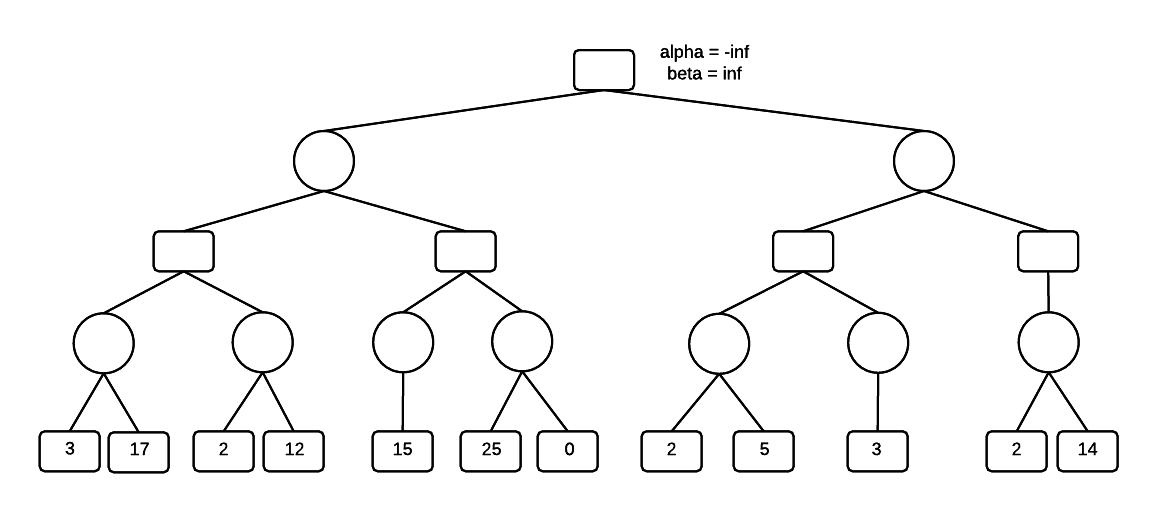
\includegraphics{./img/ABExample1_Corrected.png}

Move to the bottom of the tree, passing the values of alpha and beta all
the way down. The first player to select is MIN, and MIN will select the
minimum of its terminal-node children, which is the 3. Set beta = 3 and
leave alpha unchanged.

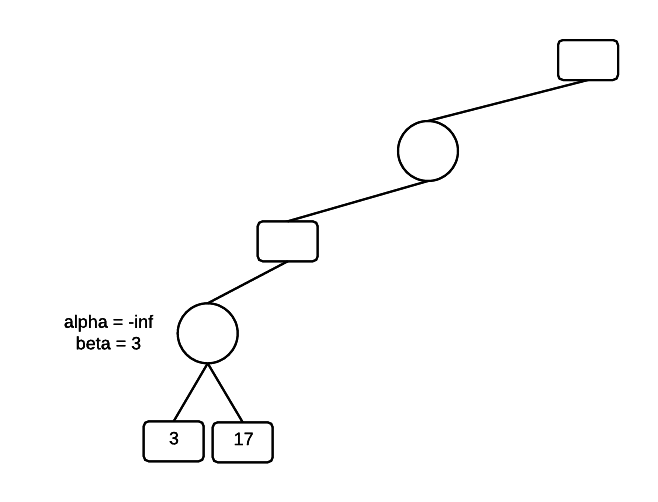
\includegraphics{img/ABExample2.png}

Next, evaluate the other child of MIN, which is the 17. Since 17
\textgreater{} 3, MIN won't select the 17 and the value of beta is
unchanged.

Once we have a MIN value, we know that MAX will be at least 3 and we can
set the minimum for MAX, alpha = 3. We've moved up a level in the tree
and there was an existing value for beta at this level. That value is
left unchanged.

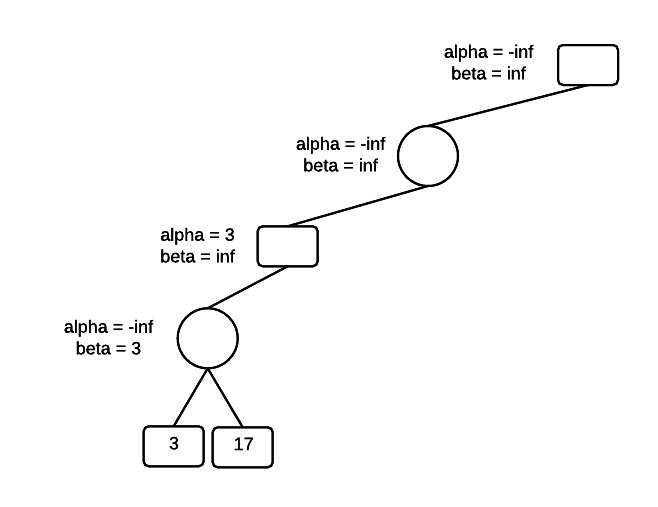
\includegraphics{img/ABExample3.png}

Next, go to the next child for MAX and traverse to the bottom of the
tree. The first node that MIN evaluates has a value of 2, which sets
beta = 2.

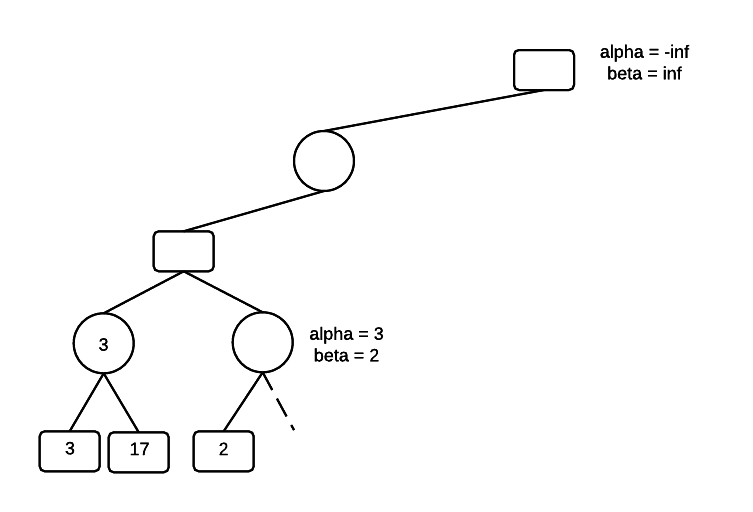
\includegraphics{img/ABExample4.png}

MIN now has a maximum value of 2. If its other children have values
higher than 2, MIN won't select them. However, MAX has a minimum value
of 3 in its other child, so MAX won't select the 2. We can prune MINs
other children and not evaluate them. We also see that the condition
alpha \textless{}= N \textless{}= beta is violated.

Set the MAX value.

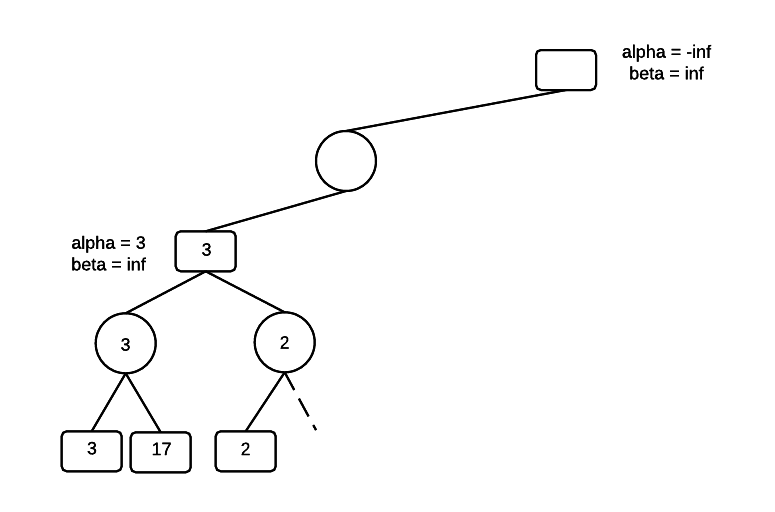
\includegraphics{img/ABExample5.png}

Move to the MIN parent node and set beta = 3. MIN might find a value
lower than 3 in the other branch of the tree, but it will not select a
value greater than 3. MIN will do no worse than 3.

Recurse to the bottom of the tree, carrying the current alpha and beta
values at each level. At the bottom of the tree, MIN encounters a value
of 15. However, beta is not changed because one of the rules of
alpha-beta pruning is that beta never increases.

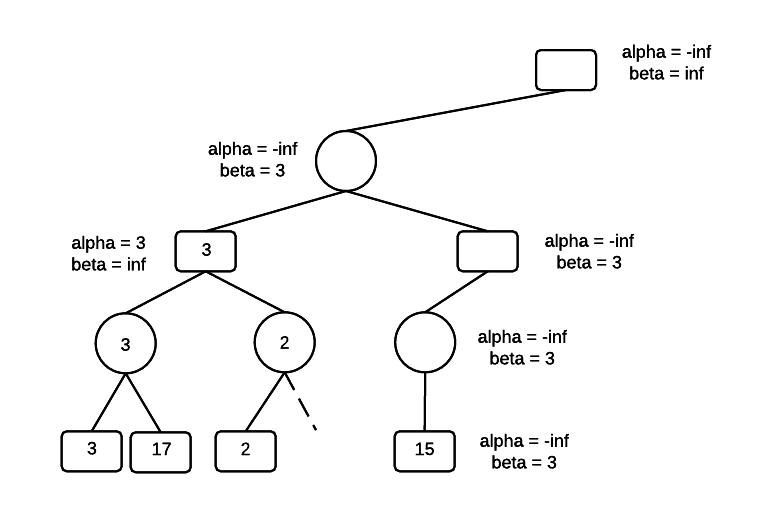
\includegraphics{img/ABExample6.png}

At the MAX level, alpha is set to 15. We now have a violation of the
constraint that alpha \textless{}= N \textless{}= beta. Also, searching
MAXs other branch is unnecessary because even if MAX finds a value
greater than 15, its MIN parent will never select it. So, the other
branch can be pruned.

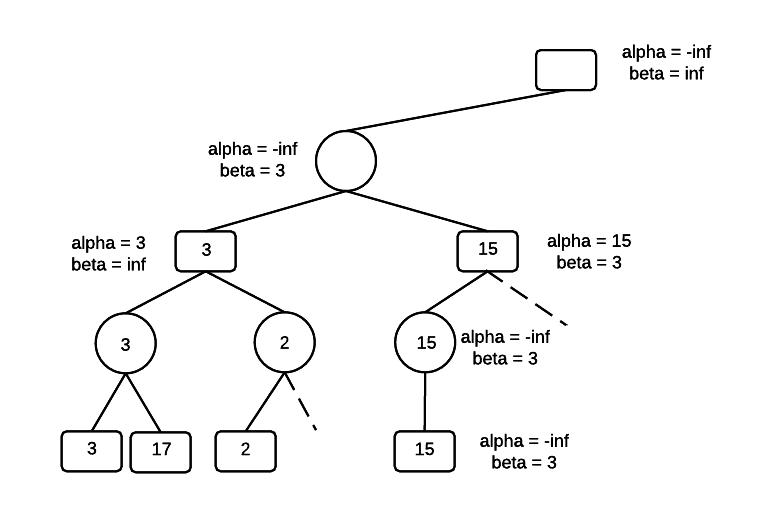
\includegraphics{img/ABExample7.png}

Assign the parent, which is a MIN node. Return to the root and set the
value for alpha. The root is a MAX node, setting alpha = 3 means that
MAX gets an outcome that is at least 3.

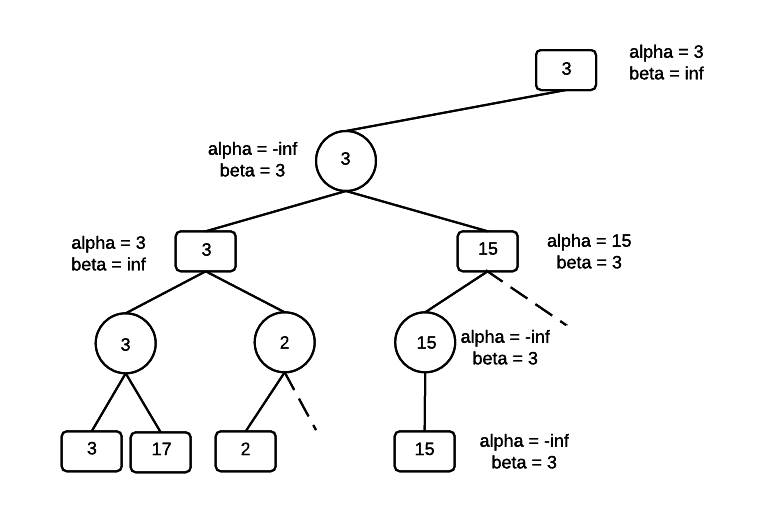
\includegraphics{img/ABExample8.png}

Traverse to the bottom of the tree, along the right branch of the root,
carrying the values for alpha and beta. At the bottom of the tree is a
value of 2 for MIN, which sets beta = 2. There is now an alpha-beta
violation and the other children of MIN can be pruned. MIN won't select
a value greater than 2 and if the 2 made it's way up the tree, it would
never be selected by MAX at the root.

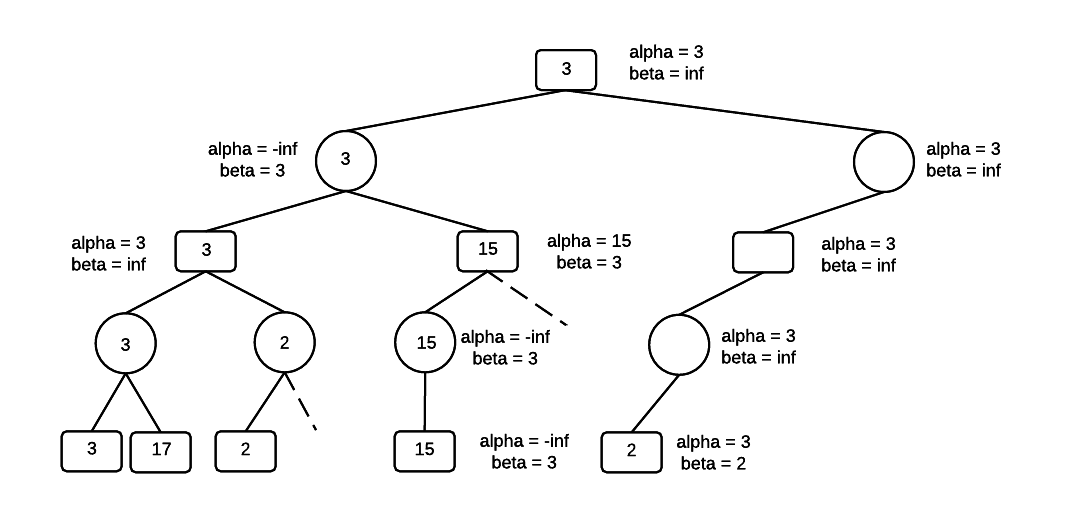
\includegraphics{img/ABExample9.png}

Set the MIN value as 2 and move up to the MAX parent level. Beta is now
2 and alpha is still 3.

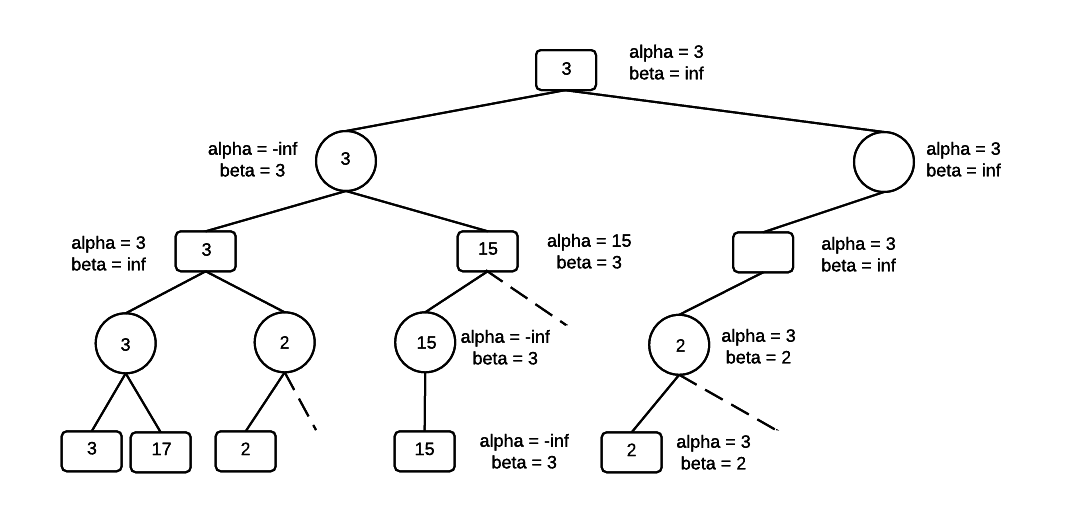
\includegraphics{img/ABExample10.png}

From the MAX level, recurse to the bottom of the tree along the right
branch, passing the values for alpha and beta all the way to the bottom
of the tree. alpha = 3 and beta = inf. The value for MIN is updated
using the value of the left-most node, which is 3. Beta is now 3, and
alpha is 3.

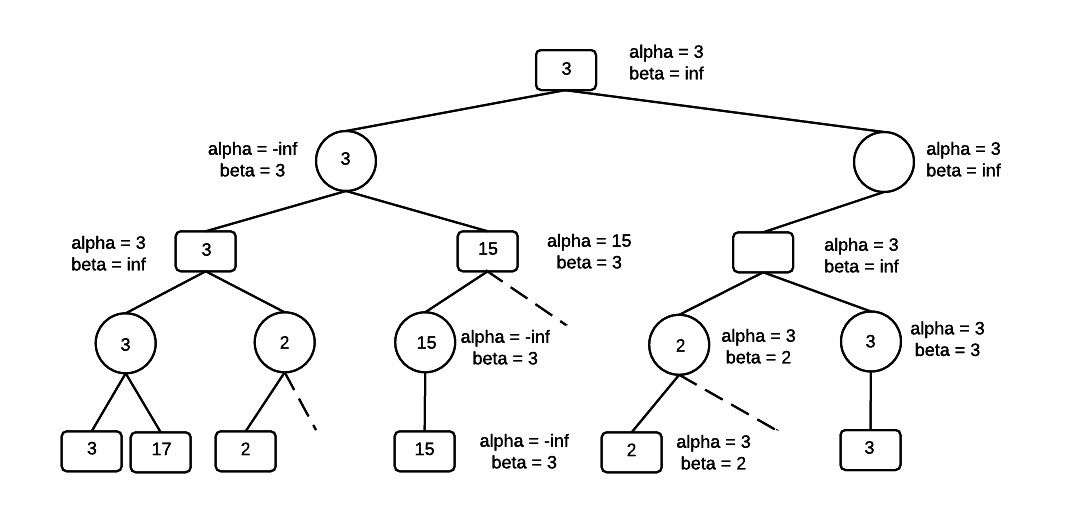
\includegraphics{img/ABExample11.png}

Move up one level in the tree to the MIN node and set beta = 3. At this
point in the algorithm, alpha = beta = 3. The remainder of the tree can
be pruned because MIN won't select a value greater than 3, and MAX at
the root, won't select a value less than 3. The search completes with a
minimax value of 3.

\begin{figure}[htbp]
\centering
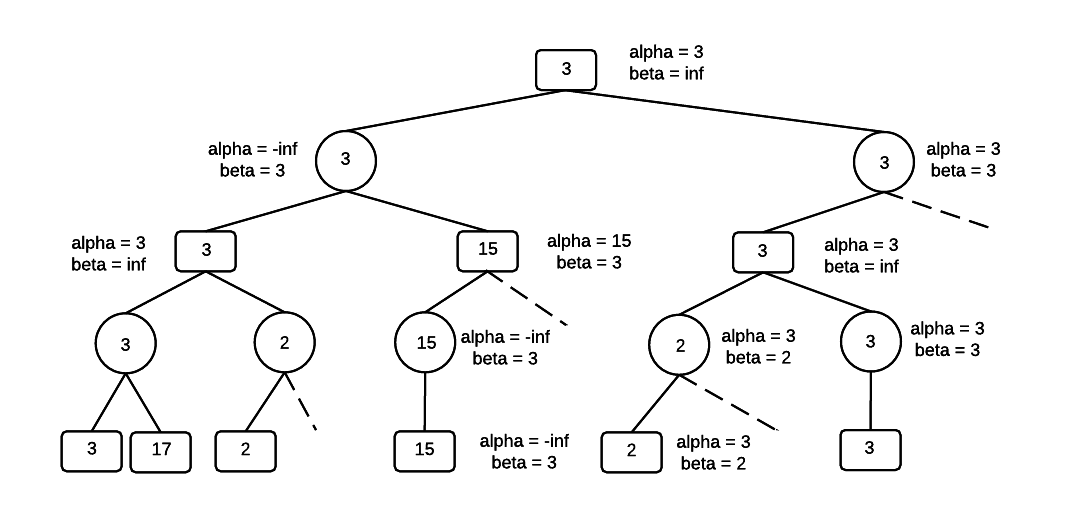
\includegraphics{img/ABExample12.png}
\caption{png}
\end{figure}

    \section{Simulated Annealing}\label{simulated-annealing}

\begin{Shaded}
\begin{Highlighting}[]
\KeywordTok{def} \NormalTok{simulated_annealing(g):}
    \NormalTok{s, c }\OperatorTok{=} \NormalTok{generate_solution(g)}
    \NormalTok{T }\OperatorTok{=} \DecValTok{1}
    \NormalTok{Tmin }\OperatorTok{=} \FloatTok{1e-9}
    \NormalTok{alpha }\OperatorTok{=} \FloatTok{0.99}
    \NormalTok{k }\OperatorTok{=} \DecValTok{1}
    \NormalTok{i }\OperatorTok{=} \DecValTok{0}
    \ControlFlowTok{while} \NormalTok{T }\OperatorTok{>} \NormalTok{Tmin:}
        \NormalTok{sp, cp }\OperatorTok{=} \NormalTok{generate_solution_neighbor(g, s, c)}
        \NormalTok{DE }\OperatorTok{=} \NormalTok{cp }\OperatorTok{-} \NormalTok{c}
        \CommentTok{# print(s, c, math.exp(-DE / (k * T)))}
        \ControlFlowTok{if} \NormalTok{DE }\OperatorTok{<} \DecValTok{0}\NormalTok{:}
            \NormalTok{s }\OperatorTok{=} \NormalTok{sp}
            \NormalTok{c }\OperatorTok{=} \NormalTok{cp}
        \ControlFlowTok{elif} \NormalTok{random.random() }\OperatorTok{<} \NormalTok{math.exp(}\OperatorTok{-}\NormalTok{DE }\OperatorTok{/} \NormalTok{(k }\OperatorTok{*} \NormalTok{T)):}
            \NormalTok{s }\OperatorTok{=} \NormalTok{sp}
            \NormalTok{c }\OperatorTok{=} \NormalTok{cp}
        \NormalTok{T }\OperatorTok{*=} \NormalTok{alpha}
        \NormalTok{i }\OperatorTok{+=} \DecValTok{1}
    \BuiltInTok{print}\NormalTok{(s, c, i)}
\end{Highlighting}
\end{Shaded}

    \section{Genetic Algorithms}\label{genetic-algorithms}

\begin{Shaded}
\begin{Highlighting}[]
\CommentTok{#!/usr/bin/env python3.5}

\ImportTok{import} \NormalTok{sys}
\ImportTok{import} \NormalTok{random}
\ImportTok{import} \NormalTok{itertools}

\NormalTok{item_count }\OperatorTok{=} \DecValTok{10}
\NormalTok{weight_limit }\OperatorTok{=} \DecValTok{50}

\CommentTok{# weight, value}
\NormalTok{items }\OperatorTok{=} \NormalTok{[(random.randint(}\DecValTok{1}\NormalTok{, }\DecValTok{15}\NormalTok{), random.randint(}\DecValTok{1}\NormalTok{, }\DecValTok{10}\NormalTok{))}
         \ControlFlowTok{for} \NormalTok{_ }\KeywordTok{in} \BuiltInTok{range}\NormalTok{(item_count)]}
\BuiltInTok{print}\NormalTok{(items)}
\BuiltInTok{print}\NormalTok{(}\StringTok{'==='}\NormalTok{)}

\NormalTok{solutions }\OperatorTok{=} \NormalTok{[}\StringTok{''}\NormalTok{.join([}\BuiltInTok{str}\NormalTok{(random.randint(}\DecValTok{0}\NormalTok{, }\DecValTok{1}\NormalTok{))}
             \ControlFlowTok{for} \NormalTok{i }\KeywordTok{in} \BuiltInTok{range}\NormalTok{(}\BuiltInTok{len}\NormalTok{(items))])}
             \ControlFlowTok{for} \NormalTok{j }\KeywordTok{in} \BuiltInTok{range}\NormalTok{(}\DecValTok{3}\NormalTok{)]}

\KeywordTok{def} \NormalTok{fitness(items, choices):}
    \NormalTok{weight }\OperatorTok{=} \DecValTok{0}
    \NormalTok{value }\OperatorTok{=} \DecValTok{0}
    \ControlFlowTok{for} \NormalTok{choice, item }\KeywordTok{in} \BuiltInTok{zip}\NormalTok{(choices, items):}
        \ControlFlowTok{if} \NormalTok{choice }\OperatorTok{==} \StringTok{'1'}\NormalTok{:}
            \NormalTok{weight }\OperatorTok{+=} \NormalTok{item[}\DecValTok{0}\NormalTok{]}
            \NormalTok{value }\OperatorTok{+=} \NormalTok{item[}\DecValTok{1}\NormalTok{]}
    \ControlFlowTok{if} \NormalTok{weight }\OperatorTok{>} \NormalTok{weight_limit:}
        \ControlFlowTok{return} \DecValTok{0}
    \ControlFlowTok{else}\NormalTok{:}
        \ControlFlowTok{return} \NormalTok{value}

\KeywordTok{def} \NormalTok{combine(choice1, choice2):}
    \CommentTok{# i = random.randint(1, item_count - 1)}
    \NormalTok{i }\OperatorTok{=} \BuiltInTok{int}\NormalTok{(item_count }\OperatorTok{/} \DecValTok{2}\NormalTok{)}
    \CommentTok{# Randomly combine}
    \ControlFlowTok{if} \NormalTok{random.random() }\OperatorTok{<} \NormalTok{.}\DecValTok{5}\NormalTok{:}
        \NormalTok{new_solution }\OperatorTok{=} \NormalTok{choice1[:i] }\OperatorTok{+} \NormalTok{choice2[i:]}
    \ControlFlowTok{else}\NormalTok{:}
        \NormalTok{new_solution }\OperatorTok{=} \NormalTok{choice2[:i] }\OperatorTok{+} \NormalTok{choice1[i:]}
    \CommentTok{# 10% of time mutate}
    \ControlFlowTok{if} \NormalTok{random.random() }\OperatorTok{<} \NormalTok{.}\DecValTok{1}\NormalTok{:}
        \NormalTok{new_solution }\OperatorTok{=} \BuiltInTok{list}\NormalTok{(new_solution)}
        \NormalTok{j }\OperatorTok{=} \NormalTok{random.randint(}\DecValTok{0}\NormalTok{, item_count }\OperatorTok{-} \DecValTok{1}\NormalTok{)}
        \ControlFlowTok{if} \NormalTok{new_solution[j] }\OperatorTok{==} \StringTok{'0'}\NormalTok{:}
            \NormalTok{new_solution[j] }\OperatorTok{=} \StringTok{'1'}
        \ControlFlowTok{else}\NormalTok{:}
            \NormalTok{new_solution[j] }\OperatorTok{=} \StringTok{'0'}
        \NormalTok{new_solution }\OperatorTok{=} \StringTok{''}\NormalTok{.join(new_solution)}
    \ControlFlowTok{return} \NormalTok{new_solution}

\KeywordTok{def} \NormalTok{gen_new(top3):}
    \NormalTok{sols }\OperatorTok{=} \NormalTok{[]}
    \ControlFlowTok{for} \NormalTok{_ }\KeywordTok{in} \BuiltInTok{range}\NormalTok{(}\DecValTok{10}\NormalTok{):}
        \NormalTok{perms }\OperatorTok{=} \BuiltInTok{list}\NormalTok{(itertools.permutations(top3))}
        \NormalTok{random.shuffle(perms)}
        \NormalTok{i, j }\OperatorTok{=} \NormalTok{perms[}\DecValTok{0}\NormalTok{][:}\DecValTok{2}\NormalTok{]}
        \NormalTok{sols.append(combine(i, j))}
    \ControlFlowTok{return} \NormalTok{sols}

\KeywordTok{def} \NormalTok{get_top3(sols):}
    \ControlFlowTok{return} \NormalTok{[s }\ControlFlowTok{for} \NormalTok{s, v }\KeywordTok{in} \BuiltInTok{sorted}\NormalTok{(get_value(sols),}
            \NormalTok{key}\OperatorTok{=}\KeywordTok{lambda} \NormalTok{tup: }\OperatorTok{-}\NormalTok{tup[}\DecValTok{1}\NormalTok{])[:}\DecValTok{3}\NormalTok{]]}

\KeywordTok{def} \NormalTok{get_value(sols):}
    \ControlFlowTok{return} \NormalTok{[(item, fitness(items, item)) }\ControlFlowTok{for} \NormalTok{item }\KeywordTok{in} \NormalTok{sols]}

\ControlFlowTok{for} \NormalTok{i }\KeywordTok{in} \BuiltInTok{range}\NormalTok{(}\DecValTok{10}\NormalTok{):}
    \BuiltInTok{print}\NormalTok{(}\StringTok{'Starting with }\SpecialCharTok{\{\}}\StringTok{'}\NormalTok{.}\BuiltInTok{format}\NormalTok{(}\BuiltInTok{str}\NormalTok{(get_value(solutions))))}
    \NormalTok{new_solutions }\OperatorTok{=} \NormalTok{gen_new(solutions)}
    \BuiltInTok{print}\NormalTok{(}\StringTok{'Birthed }\SpecialCharTok{\{\}}\StringTok{'}\NormalTok{.}\BuiltInTok{format}\NormalTok{(}\BuiltInTok{str}\NormalTok{(get_value(new_solutions))))}
    \NormalTok{full_solutions }\OperatorTok{=} \NormalTok{solutions }\OperatorTok{+} \NormalTok{new_solutions}
    \NormalTok{solutions }\OperatorTok{=} \NormalTok{get_top3(full_solutions)}
    \BuiltInTok{print}\NormalTok{(}\StringTok{'Evolved to }\SpecialCharTok{\{\}}\StringTok{'}\NormalTok{.}\BuiltInTok{format}\NormalTok{(}\BuiltInTok{str}\NormalTok{(get_value(solutions))))}
    \BuiltInTok{print}\NormalTok{(}\StringTok{'---'}\NormalTok{)}
\end{Highlighting}
\end{Shaded}

    \begin{Verbatim}[commandchars=\\\{\}]
{\color{incolor}In [{\color{incolor} }]:} 
\end{Verbatim}


    % Add a bibliography block to the postdoc
    
    
    
    \end{document}
